\documentclass{article}

\usepackage{graphicx}
\usepackage{tikz}
\usepackage{tikzsymbols}
\usetikzlibrary{calc,patterns,shapes.geometric}
\pagestyle{empty}
\usepackage[margin=0pt]{geometry}
\geometry{papersize={14in,12in}}

\def\centerarc[#1](#2)(#3:#4:#5){\draw[#1] ($(#2)+({#5*cos(#3)},{#5*sin(#3)})$) arc (#3:#4:#5);}

\begin{document}
	\begin{figure}
		\centering
		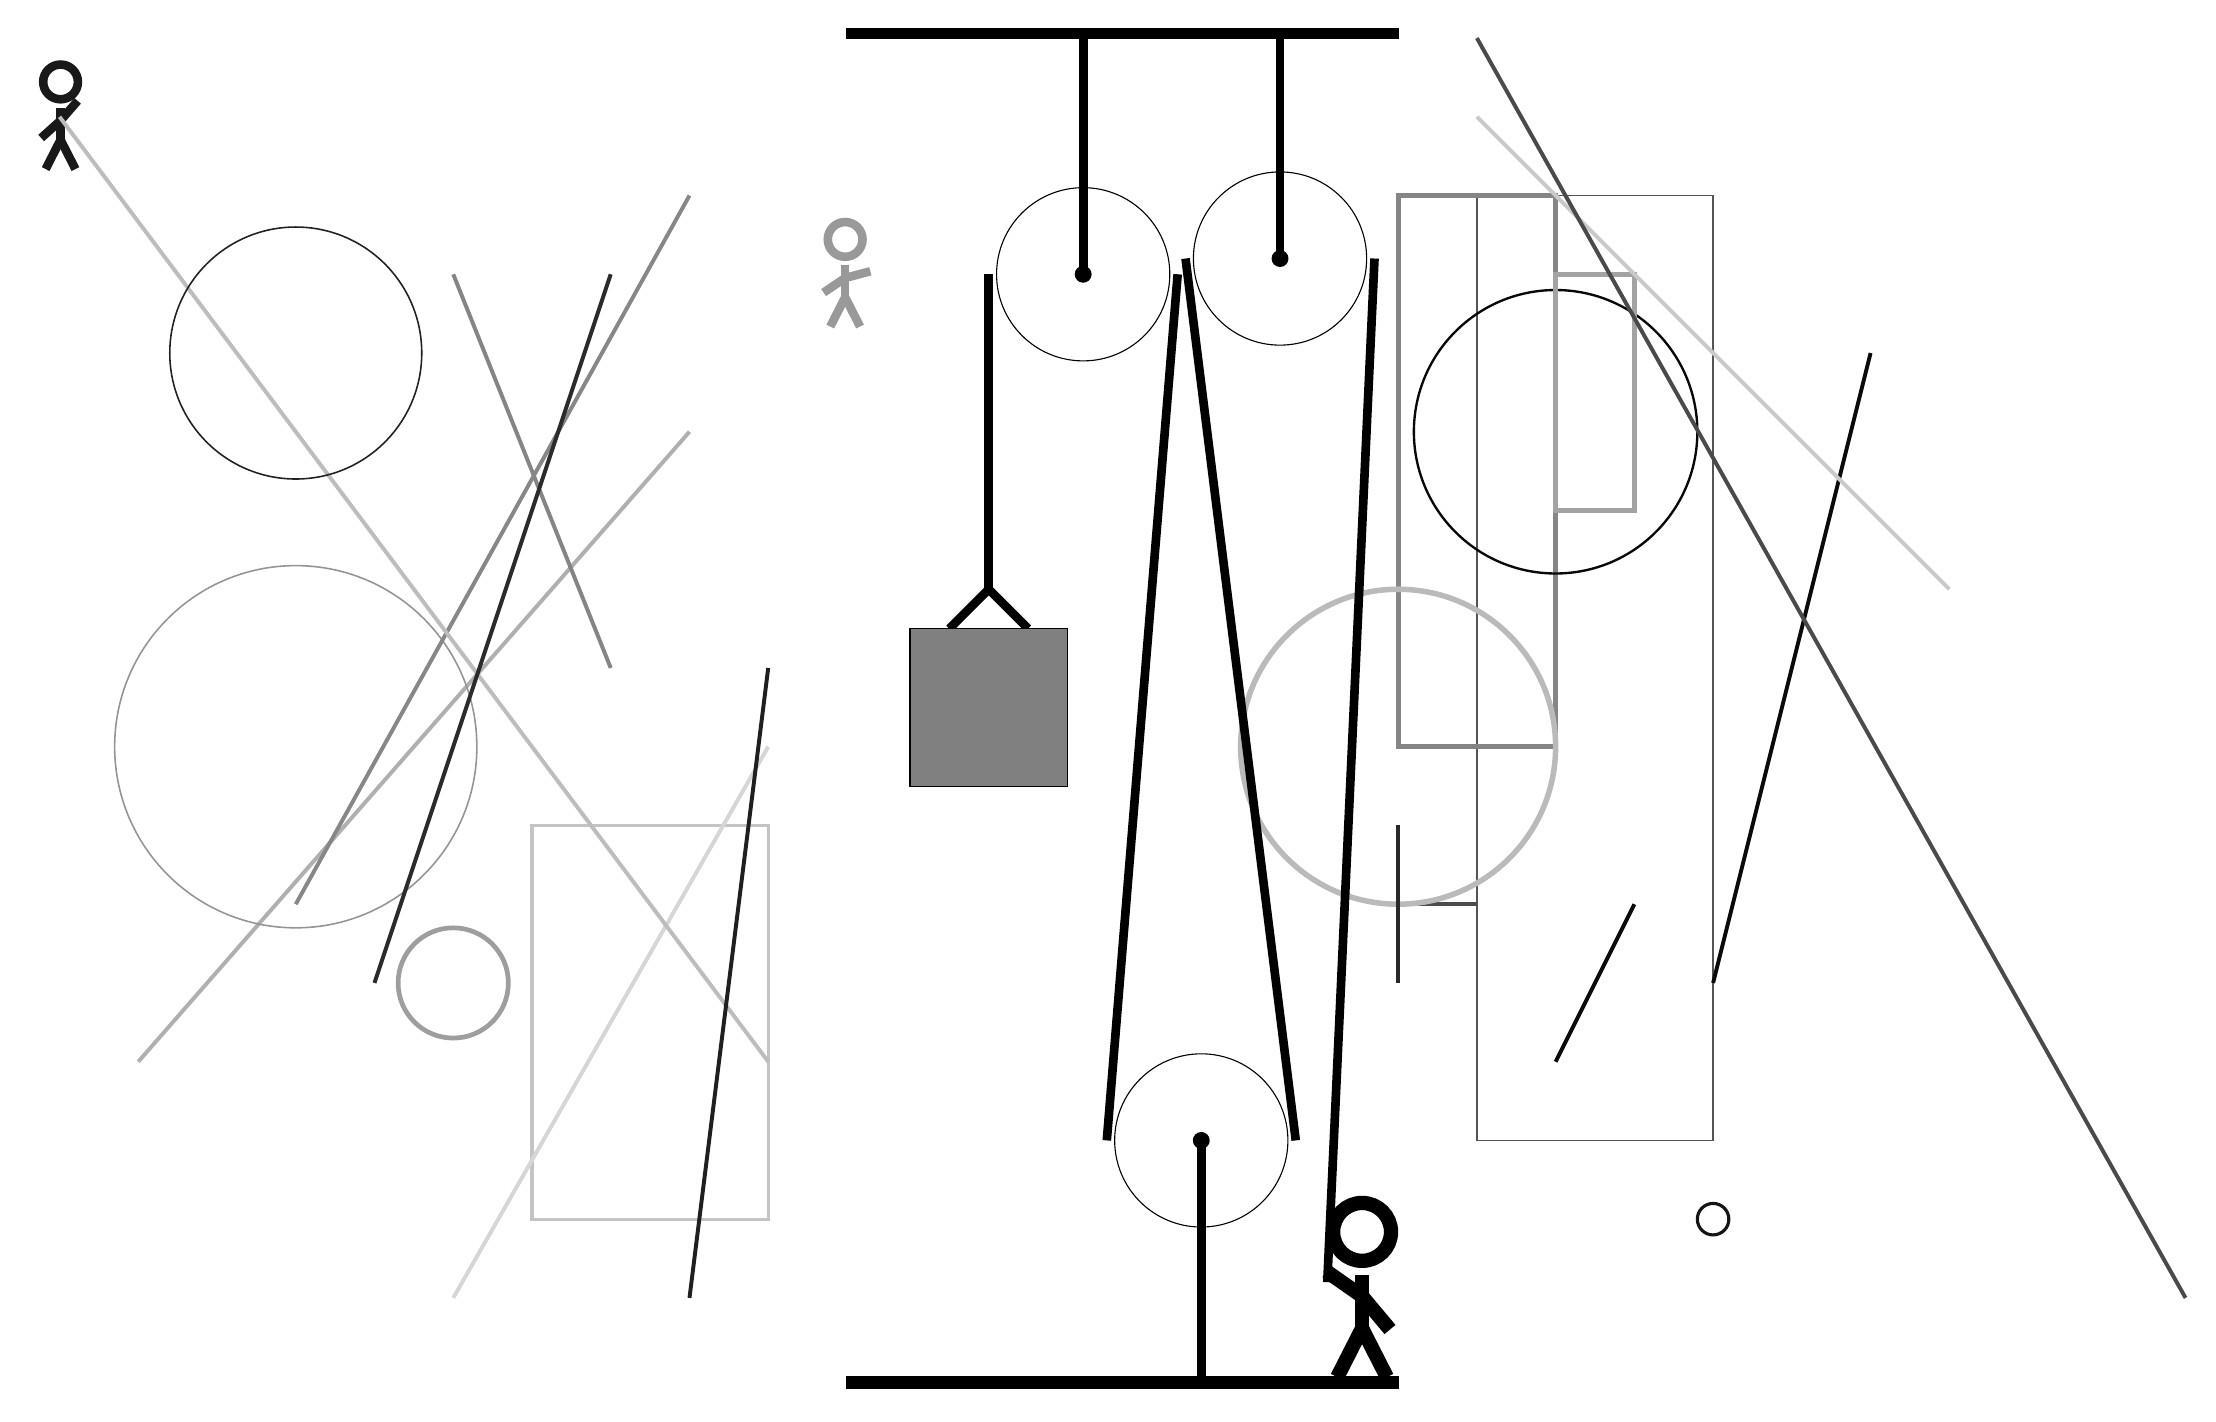
\begin{tikzpicture}
			%%%%% START %%%%%
			
			\draw[fill=black] (-2, 14) rectangle (5, 14.125);
			
			\draw (1, 11) circle (1.1);
			\draw[fill=black] (1, 11) circle (0.1);
			\draw[line width=1.1mm]  (1, 14) -- (1, 11);
			
			\draw[fill=white](2.5, 0) circle (1.1);
			\draw[fill=black] (2.5, 0) circle (0.1);
			\draw[line width=1.1mm]  (2.5, -3) -- (2.5, 0);
			
			\node[line width=0.5mm, color=black!40] at (-2, 11) {\Strichmaxerl[6][34][15]};
			
			\draw[line width=0.2mm, color=black!67] (6, 12) rectangle (9, 0);
			\draw[line width=0.5mm, color=black!31](-4, 9) -- (-11, 1);
			\draw[line width=0.5mm, color=black!48](-5, 6) -- (-7, 11);
			\draw [line width=0.6mm, color=black!38](-7, 2) circle (0.7);
			\draw[line width=0.5mm, color=black!70] (6, 3) rectangle (5, 3);
			
			\draw [line width=0.4mm, color=black!92](9, -1) circle (0.2);
			\draw[line width=0.6mm, color=black!48] (7, 5) rectangle (5, 12);
			\draw [line width=0.3mm, color=black!97](7, 9) circle (1.8);
			\draw [line width=0.2mm, color=black!42](-9, 5) circle (2.3);
			
			\draw[line width=0.4mm, color=black!23] (-3, -1) rectangle (-6, 4);
			\node[line width=0.7mm, color=black!90] at (-12, 13) {\Strichmaxerl[6][42][49]};
			\draw[line width=0.5mm, color=black!47](-4, 12) -- (-9, 3);
			
			\draw [line width=0.7mm, color=black!27](5, 5) circle (2.0);
			\draw[line width=0.7mm, color=black!36] (7, 8) rectangle (8, 11);
			\draw[line width=0.5mm, color=black!96](9, 2) -- (11, 10);
			
			\draw[line width=0.5mm, color=black!21](6, 13) -- (12, 7);
			\draw[line width=0.5mm, color=black!71](6, 14) -- (15, -2);
			\draw[line width=0.5mm, color=black!16](-3, 5) -- (-7, -2);
			\draw[line width=0.5mm, color=black!26](-3, 1) -- (-12, 13);
			\draw [line width=0.2mm, color=black!87](-9, 10) circle (1.6);
			
			\draw[line width=0.5mm, color=black!96](8, 3) -- (7, 1);
			\draw[line width=0.5mm, color=black!84](5, 2) -- (5, 4);
			\draw[line width=0.5mm, color=black!83](-5, 11) -- (-8, 2);
			\draw[line width=0.5mm, color=black!88](-3, 6) -- (-4, -2);
			
			
			\draw[fill=white](3.5, 11.2) circle (1.1);
			\draw[fill=black] (3.5, 11.2) circle (0.1);
			\draw[line width=1.1mm] (3.5, 14) -- (3.5, 11.2);
			
			\draw[line width=1.1mm] (-0.7, 6.5) -- (-0.2, 7.0) -- (0.3, 6.5);
			\draw[fill=black!50] (-1.2, 6.5) rectangle (0.8, 4.5);
			
			\draw[line width=1.1mm] (-0.2, 11) -- (-0.2, 7.0);
			\centerarc[line width=1.1mm](1, 11)(0:180:1.2000000000000002);
			\draw[line width=1.1mm](2.2, 11) -- (1.3, 0);
			\centerarc[line width=1.1mm](2.5, 0)(180:360:1.2000000000000002);
			\draw[line width=1.1mm](3.7, 0) -- (2.3, 11.2);
			\centerarc[line width=1.1mm](3.5, 11.2)(0:180:1.2000000000000002);
			\draw[line width=1.1mm](4.7, 11.2) -- (4.1, -1.8);
			
			\node at (4.5, -1.9) {\Strichmaxerl[10][-35][-50]};
			
			\draw[fill=black] (-2, -3) rectangle (5, -3.15);
			
			%%%%% END %%%%%
		\end{tikzpicture}
	\end{figure}	
\end{document}